\documentclass[12pt]{article}

\usepackage[margin=1in]{geometry} 
\usepackage{amsmath,amsthm,amssymb}
\usepackage[spanish]{babel}
\usepackage[utf8]{inputenc}
\usepackage{tikz-cd}
\usepackage{amsmath}
\usepackage[shortlabels]{enumitem}
\usepackage{mathtools}
\usepackage{float}

\title{SWAP: Práctica 1}
\author{
        Antonio Gámiz Delgado
}

\begin{document}
\maketitle



Instalamos y configuramos la máquina \textbf{M1}:

\begin{figure}[H]
  \center
  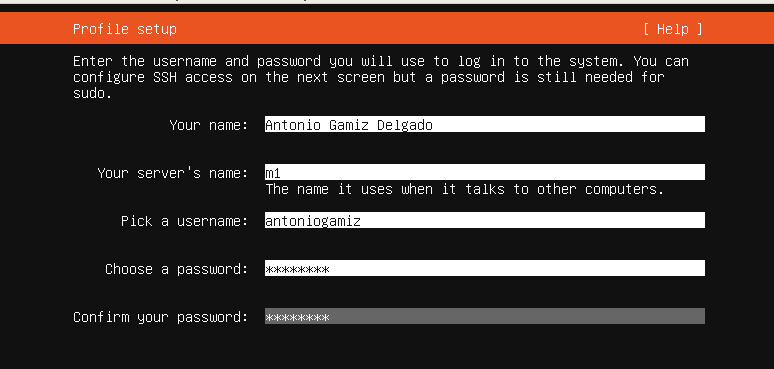
\includegraphics[scale=0.5]{img/1.png}
\end{figure}

Instalamos y configuramos la máquina \textbf{M2}:

\begin{figure}[H]
  \center
  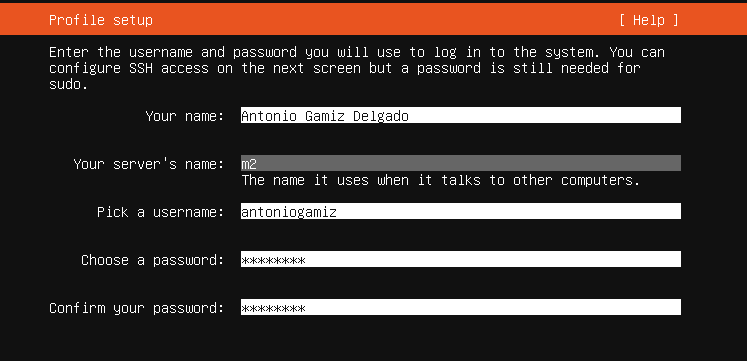
\includegraphics[scale=0.5]{img/2.png}
\end{figure}

A partir de ahora solo pondré fotos de una de las máquinas (la otra se hace igual). 

\newpage

Creamos las tarjetas de red:

\begin{figure}[H]
  \center
  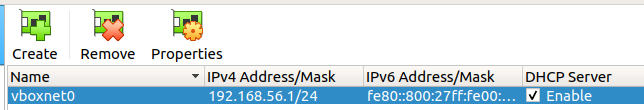
\includegraphics[scale=0.5]{img/113.png}\\
  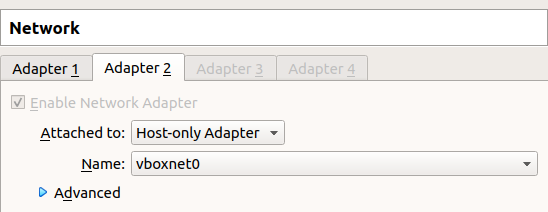
\includegraphics[scale=0.5]{img/114.png}
\end{figure}

Nos conectamos mediante \textit{ssh} a \textbf{M1}:

\begin{figure}[H]
  \center
  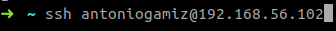
\includegraphics[scale=0.5]{img/3.png}
\end{figure}

Configuramos el entorno de red:

\begin{figure}[H]
  \center
  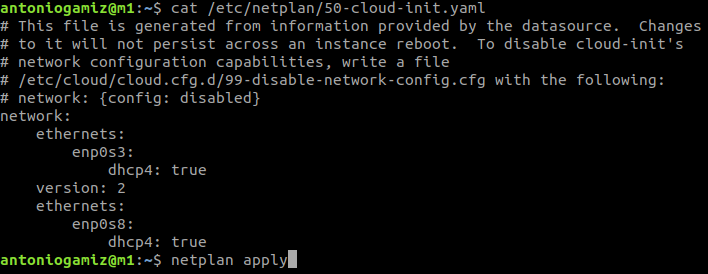
\includegraphics[scale=0.5]{img/111.png}
\end{figure}

Ahora instalamos todas las dependencias necesarias:

\begin{figure}[H]
  \center
  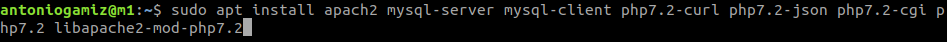
\includegraphics[scale=0.5]{img/112.png}
\end{figure}

Comprobamos el correcto funcionamineto de \textit{Apache2}:

\begin{figure}[H]
  \center
  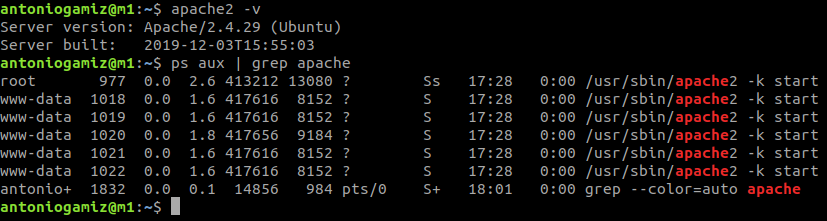
\includegraphics[scale=0.5]{img/115.png}
\end{figure}

Añadimos una página web básica y comprobamos que se sirve correctamente:

\begin{figure}[H]
  \center
  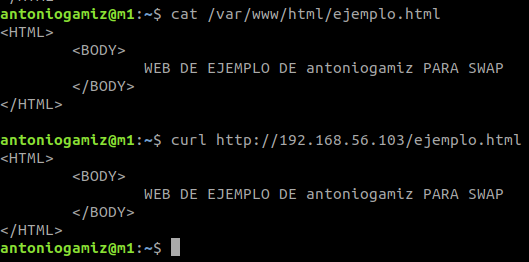
\includegraphics[scale=0.5]{img/116.png}
\end{figure}

\end{document}
